\section{Temporal analysis}
\label{sec:chap_lidar_temporal}

In this section, we analyze the temporal behavior of the four sensors for the duration of six complete snowstorms. In particular, we are interested in seeing how the fraction of echoes in snowflakes evolves over time, for all four sensors. First, we will discuss the highly dynamical nature of snowstorms. This will be exemplified by how consecutive scans can have significant quantitative and spatial differences in the distributions of the snowflakes echoes, which justify the use of averaging windows for our analysis. We will then present the actual temporal evolution of these statistics in the form of graphs for all four sensors, and finally briefly discuss the results for each sensor.

\subsection{Extraction of temporal statistics}

Snowstorms are highly dynamic processes, with large variation in snowfall rates over their durations. Moreover, the snow physical characteristics (size, shape or reflectance) might vary significantly during a storm, affected by ambient conditions such as humidity level and temperature. Also, wind gusts might pull snow back up in the air or drive it sideways, affecting its effective fall rate. Consequently, one expects during a snowstorm to see significant short, medium and long term variations in the fraction of LiDAR echoes corresponding to the falling snow.

Computing and reporting the temporal statistics for every scan would put too much emphasis on the very short-term statistics. Indeed, the inter-scan variation in the fraction of snowflake echoes can be significant. To better illustrate this point, we have overlaid four consecutive scans in the same plot for the LMS200 and for the first echo returned by the multi-echo Hokuyo sensor in Figure~\ref{fig:LMS200_4Scans_Feb19}, for an intense snowing episode from the 02-19 dataset (see Table~\ref{tab:overview-dataset}). In these figures, we can see strong variations in the fraction of snowflake echoes and their spatial distribution, which we believe can be best described as a random process. One can readily see the fluctuation in these fractions as reported in the brackets of the legend in Figure~\ref{fig:LMS200_4Scans_Feb19}.

To smooth out these fluctuations, statistics are extracted from a number of consecutive scans contained in a time window of around 1~minute (detailed values in Table~\ref{tab:selectionScans}). Figure~\ref{fig:TimingSnow} shows this smoothed fraction of snowflake echoes compared to all returned laser measurements as a function of time, for the six snowiest days of our dataset. To allow for better visualization, only the LMS200 and the Hokuyo's first echo are plotted at their actual scale (1x): Others have been scaled up (from 30x to 200x), with their corresponding scaling factors reported in the legend. As will be shown below, some sensors were much more sensitive than others.

\begin{figure}[h]
    \centering
    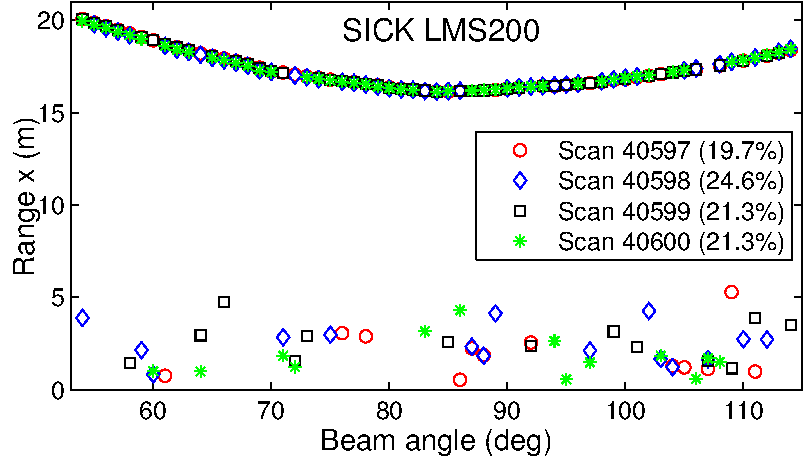
\includegraphics[trim={0.2cm 0 0 0},clip,width=0.7\linewidth]{./img/chap_lidar/LMS200_4Scans_Feb19.pdf}
    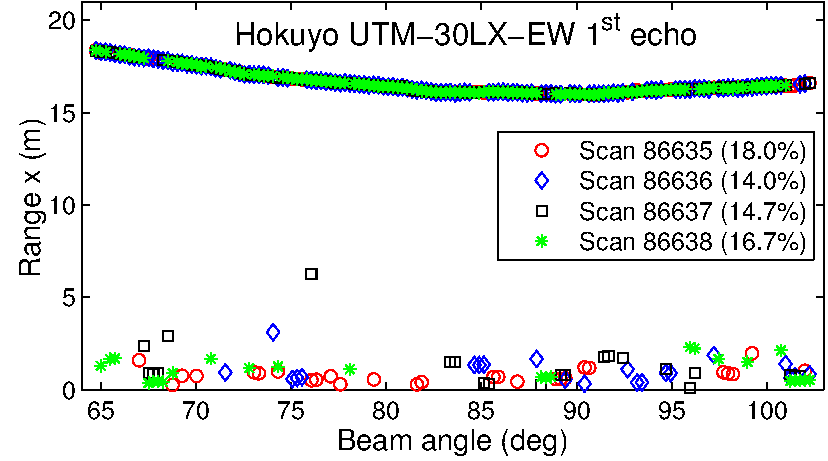
\includegraphics[trim={0.2cm 0 0 0},clip,width=0.7\linewidth]{./img/chap_lidar/Hokuyo_4Scans_Feb19.pdf}
    \caption{Four overlaid consecutive scans for the LMS200 sensor (top), and the first echo scans for the Hokuyo sensor (bottom), taken from the 02-19 dataset. Each symbol corresponds to a particular scan. The curved line at the top corresponds to the snow surface on the ground. One can see the rapid variation of the snowflake echoes between scans, and how they are mostly limited to a range $x<\SI{5}{\meter}$. The percentages (in brackets) are the proportion of those echoes in the snowflakes.}
    \label{fig:LMS200_4Scans_Feb19}
\end{figure}

\subsection{Detailed analysis, per sensor}

\subsubsection{SICK Sensors LMS200 and LMS151}
Our first conclusion based on Figure~\ref{fig:TimingSnow} is that the most sensitive device was the older LMS200, first introduced in the mid-2000s. For the most intense snowstorms (Figure~\ref{fig:TimingSnow}. b) 02-19, d) 03-17, e) 03-21 and f) 03-30), it peaked at around 15\% of measurements triggered by the falling snowflakes, for averaging windows of \SI{106}{\second}. As an older-generation device, it probably uses less sophisticated algorithms and sensing, and was not directly targeted for harsh outdoor environments. Indeed, its technical description~\cite{LMS200Manual} indicates that ``Raindrops and snow-flakes are cut out using pixel-oriented evaluation'', but this seems only applicable to obstacle detection (field computation), not the actual measurements. No further details are given. On the other hand, the more recent SICK LMS151 exhibits much less sensitivity to snowflakes: The reduction factor for the fraction of snowflakes echoes is in the order of 200-300, granting this device a much higher immunity in snowstorms. Indeed, the highest peak was around 0.1 \% of echoes in snowflakes during the 02-19 dataset. In some sense, this is not surprising considering that the documentation from the manufacturer mentions that this model is targeted for ``all weather conditions''~\cite{LMS151Manual}.

%Advances in optics and algorithms are probably responsible for this significant improvement~\todo{sounds too generic and hypothetical. Remove?}. Moreover, this device can be programmed to return either the first or second echo\todo{Make sure this information is ok.}. In our tests, we selected the latter: it would have been however interesting to perform tests to get information about the first echo, but our current system was not capable of gathering this information.

\begin{figure}[h]
    \centering
    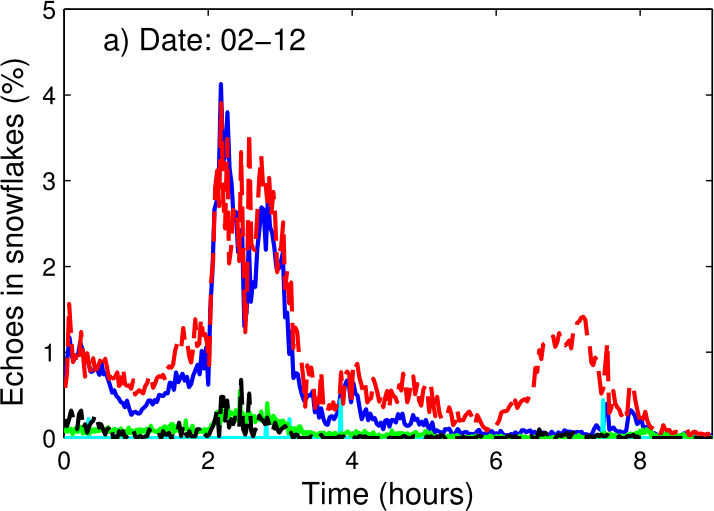
\includegraphics[width=0.45\linewidth]{./img/chap_lidar/timings_cropped_a.png}
    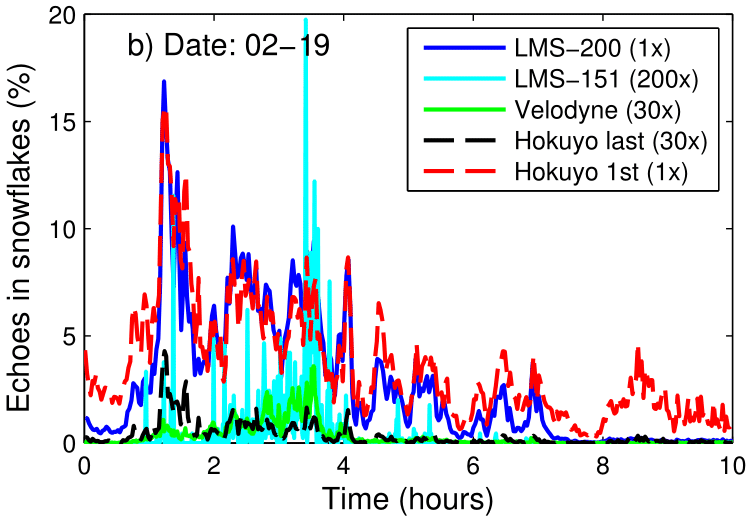
\includegraphics[width=0.45\linewidth]{./img/chap_lidar/timings_cropped_b.png}
    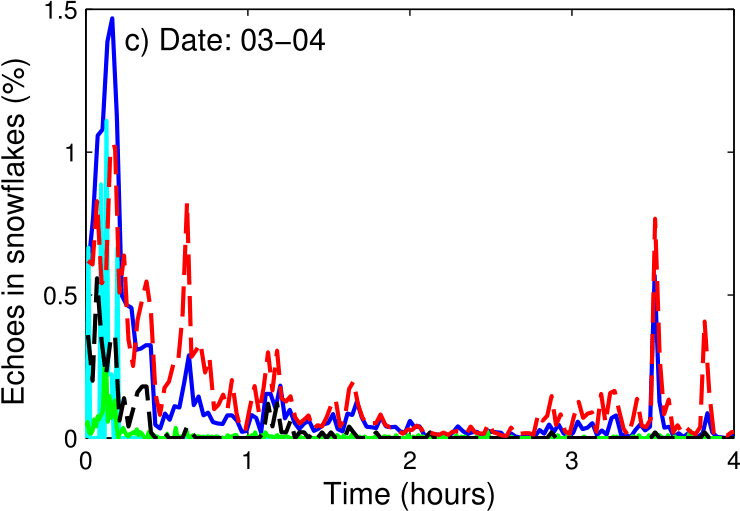
\includegraphics[width=0.45\linewidth]{./img/chap_lidar/timings_cropped_c.png}
    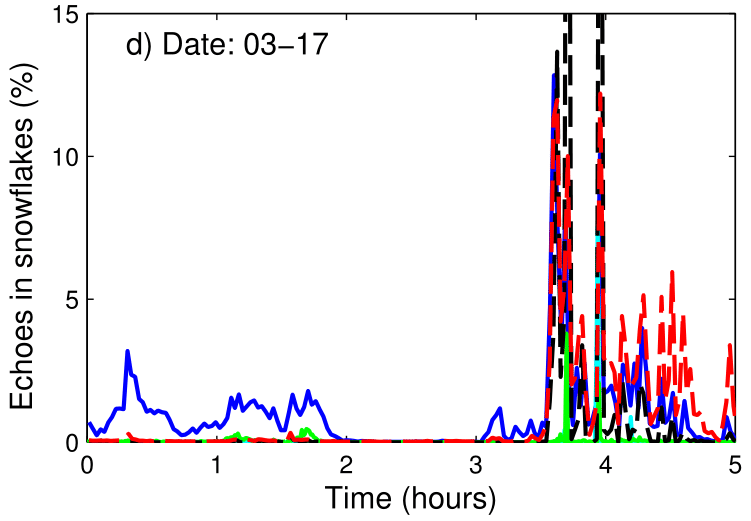
\includegraphics[width=0.45\linewidth]{./img/chap_lidar/timings_cropped_d.png}
    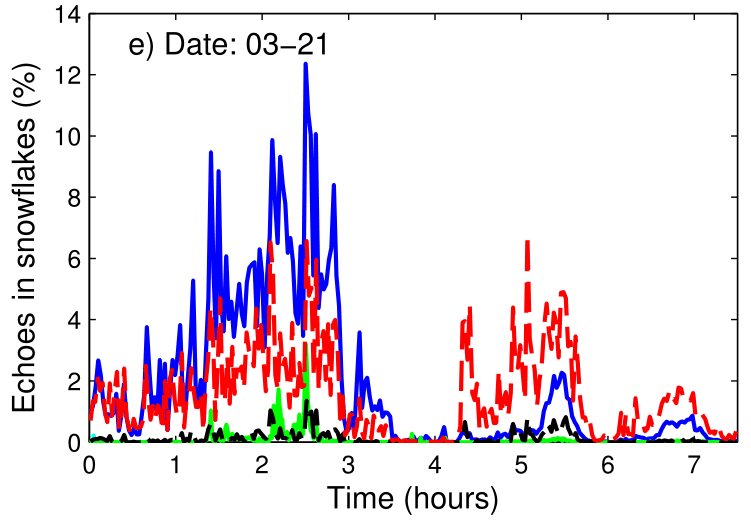
\includegraphics[width=0.45\linewidth]{./img/chap_lidar/timings_cropped_e.png}
    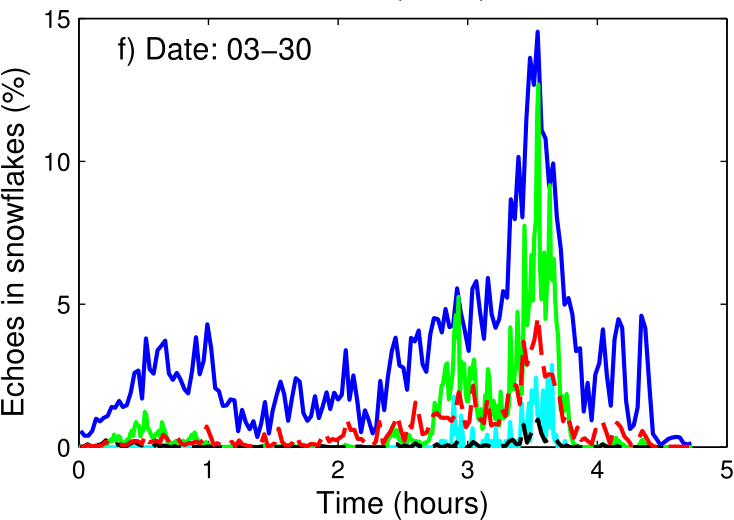
\includegraphics[width=0.45\linewidth]{./img/chap_lidar/timings_cropped_f.png}
    \caption{Temporal evolution of the percentage of echoes coming from the falling snow (range $x<$\SI{5}{\meter}) during the 6 most intense episodes, for all 4 sensors. The data is smoothed by taking statistics for small time windows. Except for the LMS200 and Hokuyo first echo, all other sensors statistics have been scaled up (factor in bracket of legend b) for ease of visual comparison. Time is in hour, starting from the beginning of the data capture sequence.}
    \label{fig:TimingSnow}
\end{figure}


\subsubsection{Hokuyo UTM-30LX-EW}
For this sensor, we resorted to a slightly different approach for comparison, as the device has been designed to return multiple echoes. We thus extracted statistics for the two most relevant cases: for first and last echoes. Statistics for the first echo tells us how sensitive the device is, if one wishes to detect the presence or absence of falling snow. This information could be used, in turn, to adapt the driving strategy of an autonomous vehicle or inform vision algorithms of the presence of particles in the air. On the other hand, using the last echo increases the probability that we will detect obstacles, such as another vehicle or the snow-covered ground. This information would be used for localization and navigation purposes. In the case of the first echo, we observed that the device behaved similarly to the LMS200. Indeed, the Hokuyo first echo (blue line) closely tracks the LMS200 curves (red dashed line) almost everywhere in Figure~\ref{fig:TimingSnow}, with a few exceptions.  In the case where we look at the last echo, the sensor behaves like the LMS151, not surprisingly as this sensor does a 2-echoes analysis and filtering. The last echo of the Hokuyo tends to reject the falling snow, but not as well as the LMS151, as it peaked at around 0.5~\% in some episodes. Nevertheless, this difference might not be sufficient to impact algorithms relying on laser data. Note that Table~\ref{tab:avgRates} shows similar correlations between these three sensors, for the averages taken over the complete 02-19 dataset.

\begin{table}[h]
    \centering
    \begin{tabular}{@{}rrrrr@{}}
        \toprule
        \textbf{LMS200} & \textbf{Hokuyo first echo}     & \textbf{Hokuyo last echo}    & \textbf{LMS151} & \textbf{Velodyne HDL-32E} \\
        \hline
        2.67\%          &           3.55\%    &       0.0113\%     &   0.00178\%     &  0.0100\%  \\
        \bottomrule
    \end{tabular}
    \caption{Overall average snowflake echoes for the complete 02-19 dataset, per sensor. These averages are significantly lower than the instantaneous values displayed in Figure~\ref{fig:TimingSnow}, as snow was not falling at all times during that period.}
    \label{tab:avgRates}
\end{table}

\subsubsection{Velodyne HDL-32E}
For all purposes, the behavior of the Velodyne was similar to the last echo of the Hokuyo sensor. This is seen both in the temporal behavior in Figure~\ref{fig:TimingSnow} and in the average value displayed in Table~\ref{tab:avgRates}.

% ========================= Histograms ===================
\section{Distribution of snowflake echoes as a function of range}
\label{sec:chap_lidar_histo}

In the previous section, we showed how the expected fraction of snowflake echoes varied temporally during snowstorms. In some sense, it provided for a \emph{temporal} modeling of the interaction between a snowstorm and a given LiDAR. In this section, we evacuate the temporal aspect and instead focus on how the range $x$ affects the probability for a snowflake to trigger a measurement. To this end, we will use histograms to estimate a probability density function of those events, and show that for the weather condition and the sensors we tested, there seems to be an upper bound on the range $x$ beyond which falling snowflakes no longer trigger a measurement: In other words, snowflakes become invisible to the sensor past a certain range.

\subsection{Modeling the impact of range on snowflake detection}
When modeling a range sensor, one has to have an idea of the probability distribution of certain events (e.g. snowflakes) as a function of this range. Over the years, many researchers have proposed probabilistic models for sensors, notably in Thrun et al.~\cite{Thrun:2005:PR:1121596}. In the previous section, we have in some sense estimated the probability for a given sensor S that a snowflake would generate an echo $E_\text{snowflake}$ given the weather condition $W$, or $P_S(E_\text{snowflake}|W)$. In this section, we take a closer look at which range $x$ such events would be generated, that is $P_S(E_\text{snowflake}|x,W)$. Having such a formulation would allow for a more statistically-sound treatment of the information, such as within a Bayesian probabilistic framework. To this effect, we use histograms as approximations to the previous distribution. In Figure~\ref{fig:Histograms}, we have plotted these histograms for each of the four sensors. For ease of comparison, they have all been normalized by their total area in the interval $0 < x < \SI{14}{\meter}$, as the total count varies widely between the sensors. The numbers in brackets in the legend indicate the fraction of echoes in the snowflakes compared to the total number of data points, for a given dataset.

%, such as
%\begin{equation}
%p(e|x,w)=p(e|w)p(e|x)
%\end{equation}
%where p(e|x) would be the log-normal distribution and p(e|w) the probability of having snow affecting

The general shape of these histograms is close to a log-normal distribution, with the exception of the LMS200 for a number of dates (02-12 through 03-17), which seems to follow a sum of two log-normal distributions. We attribute this log-normal shape to the interaction between two different phenomena, illustrated in a cartoon-type model in Figure~\ref{fig:CartoonModel}. At short ranges $x<\SI{3}{\meter}$, the building acts as a shield and decreases the probability of having a snowflake in the path of the laser. We recognize that this phenomenon would be most likely absent on an autonomous vehicle, thereby increasing the probability of having echoes in snowflakes at close range. However, we believe that this difference is not problematic, as close obstacles would be easily detected from \emph{i)} the overwhelming number of  LiDAR echoes on this obstacle \emph{ii)} other sensing modalities such as vision or radar. Furthermore, if the LiDAR is to be mounted on a rooftop, one can safely  ignore echoes in the first \SI{2}{\meter}, either in software or directly through the sensor itself (via its configuration). The other phenomenon, illustrated as the red dashed line in Figure~\ref{fig:CartoonModel}, is the probability of optical detection of a snowflake by the sensor as a function of the range $x$. We argue that this shape is due to the rapidly decreasing light intensity of the echoes in snowflakes, as a function of $x$. Combining these two phenomenon yields a log-normal shaped curve (black line in Figure~\ref{fig:CartoonModel}). Overall, this seems to indicate that a simple probabilistic model $P_S(E_\text{snowflake}|x,W)$ can be derived for these sensors.

\begin{figure}[h]
    \centering
    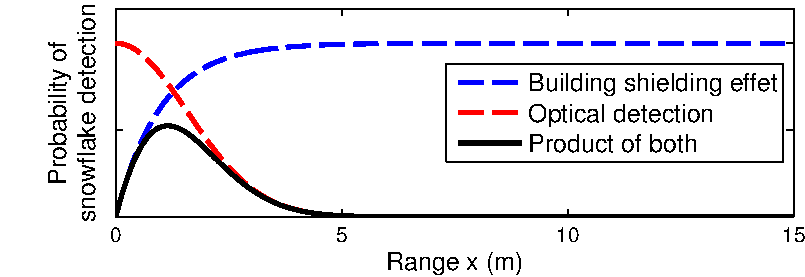
\includegraphics[trim={0.6cm 0 0 0},clip,width=0.7\linewidth]{./img/chap_lidar/ShieldingModel.pdf}
    \caption{Cartoon representation of the interaction between the probability of detecting a snowflake (in red) and the diminution of snowflakes due to the shielding effect of the building (in blue). The black line is the product of the two, and bear a close resemblance to the actual histograms extracted from our dataset.}
    \label{fig:CartoonModel}
\end{figure}


\subsection{Sensor results}
As can be seen from the histograms in Figure~\ref{fig:Histograms}, most sensors exhibit the log-normal or sum-of-log-normal distributions discussed above. We note that for certain days, the distributions are shifted to the right (greater range $x$). In particular, for the 03-21 and the 03-30 distributions, this shift is substantial (on the order of \SI{1}{\meter}). We suspect that for these days, the snowflakes were significantly larger, thus allowing for a stronger optical echo and extended range of detection.

For all sensors, we can also conclude that beyond the range $x>\SI{10}{\meter}$, snowflakes are no longer detected, i.e. they become invisible. A small notable exception would be for the Velodyne, for which snowflakes were detected all the way to $x=\SI{14}{\meter}$, albeit at a significantly reduced rate. Again, we do not think that this would significantly impair their use in conditions similar to our test setup.

%Note that for the LMS151, the amount of data was not sufficient to draw much conclusion on this distribution except for the fact that there was virtually no events passed 4.

\begin{figure}[h]
    \centering
    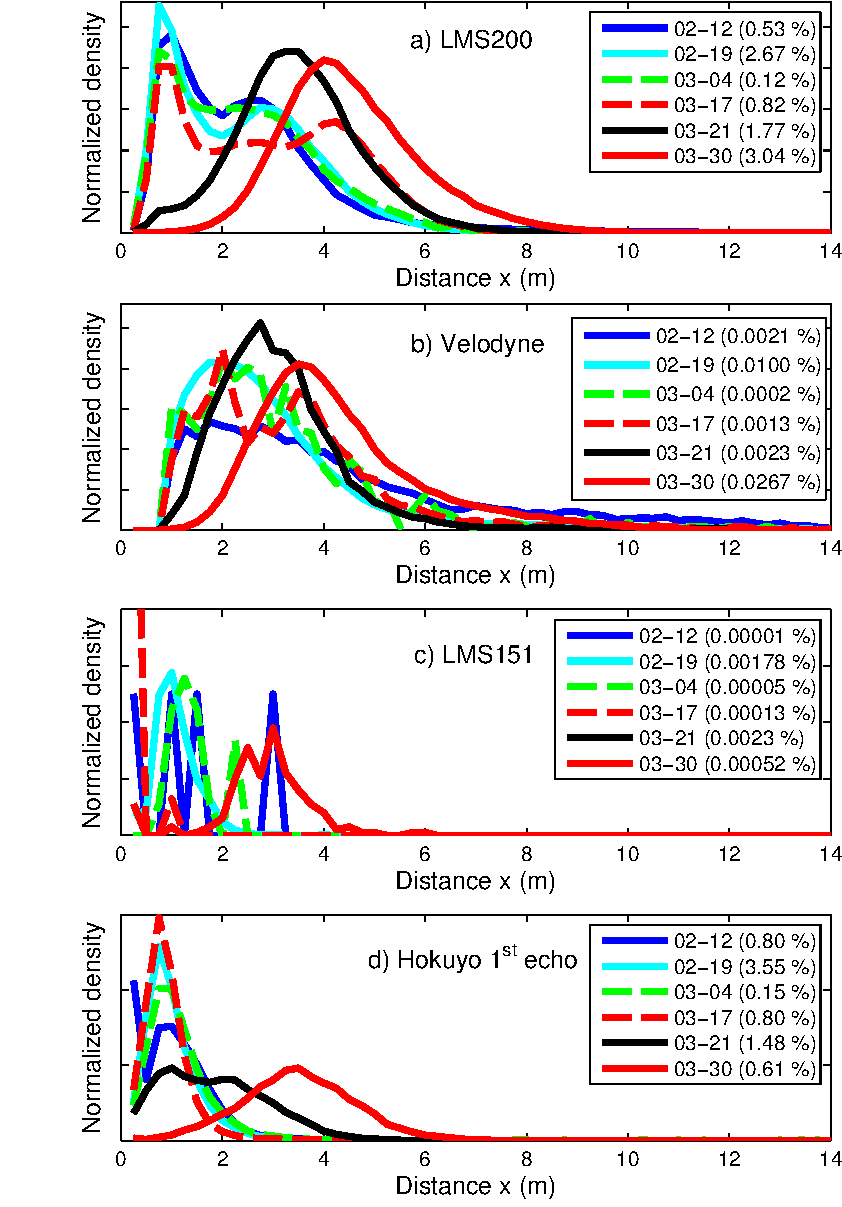
\includegraphics[trim={1.1cm 0 0 0},clip,width=0.80\linewidth]{./img/chap_lidar/Histogram.pdf}
    \caption{Histograms of echoes in falling snow during important snowfall days, as a function of distance $x$ reported by the sensor. Each histogram has been normalized by its area, for ease of comparison. The numbers in brackets are the fraction of data points in the complete dataset that correspond to snowflake echoes. Note that for the 03-21 dataset, the LMS151 was not working properly: thus no data is included for that day.}
    \label{fig:Histograms}
\end{figure}
